%\begin{sidewaysfigure}
%  \begin{center}
%  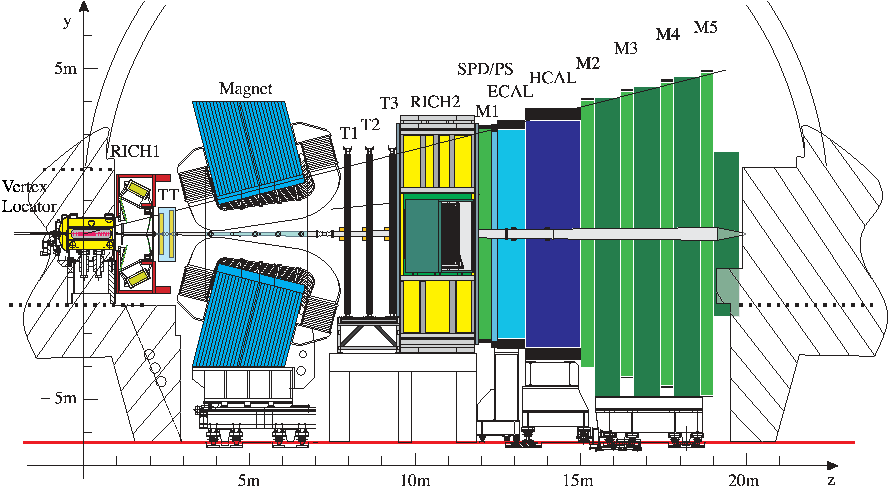
\includegraphics[width=0.8\textheight]{lhcb-detector-cross-section}
%  \caption[Cross-section view of \LHCb, cut in the non-bending $y$--$z$ plane]%
%    {Cross-section view of \LHCb, cut in the non-bending $y$--$z$ plane.}
%  \label{fig:LHCbCrossSection}
%  \end{center}
%\end{sidewaysfigure}



\chapter{The T2K Experiment}
\label{chap:T2KExperiment}
\begin{figure}
  \centering
  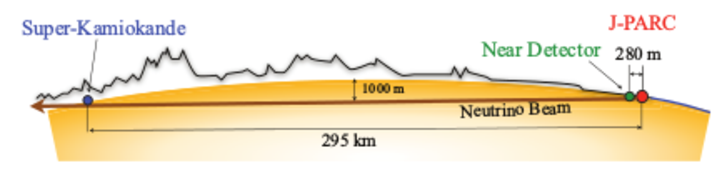
\includegraphics[width=10cm]{images/t2k/t2k_schematic.pdf}
  \caption{The T2K experiment.}
  \label{fig:T2KSchematic}
\end{figure}


The Tokai-to-Kamioka (T2K) experiment~\cite{Abe2011106} is a long baseline neutrino oscillation experiment located in two sites across Japan which was designed to study the parameters governing the PMNS matrix.  The first site is the J-PARC facility in Tokai-mura on Japan's east cost which houses a 30 GeV proton accelerator complex that is used to generate a highly pure $\nu_\mu$ beam.  J-PARC also contains a suite of detectors designed to measure the neutrino beam's unoscillated characteristics.  Super-Kamiokande (SK) is located 295 km (see Fig.~\ref{fig:T2KSchematic}) and measures the contents of the neutrino beam post-oscillation.
\newline
T2K was the first experiment to observe the $\nu_\mu\rightarrow\nu_e$ appearance channel~\cite{PhysRevLett.112.061802} which excluded $\theta_{13} = 0$ at 7.3$\textrm{\sigma}$ significance.  By comparing this result with precise $\theta_{13}$ measurements from reactor experiments, $\textrm{\delta}_{\textrm{CP}}$ regions can be excluded at 90$\%$ confidence level (see Fig.~\ref{fig:NueAppearanceContour}).  T2K's precision analysis of the $\nu_\mu$ disappearance channel provide world leading measurements of $\textrm{\theta}_{23}$ and $\Delta m^2_{23}$.  Independently of the oscillation analyses performed by the experiment, T2K's near detectors, ND280 and INGRID, are used to measure a range of neutrino cross-sections~\cite{PhysRevLett.113.241803, PhysRevD.87.092003}.  While this is not the primary aim of T2K, such measurements are still extremely important as T2K systematic uncertainties can be constrained with additional cross-section knowledge as well as helping to understand the general neutrino interaction picture.

\begin{figure}
  \centering
  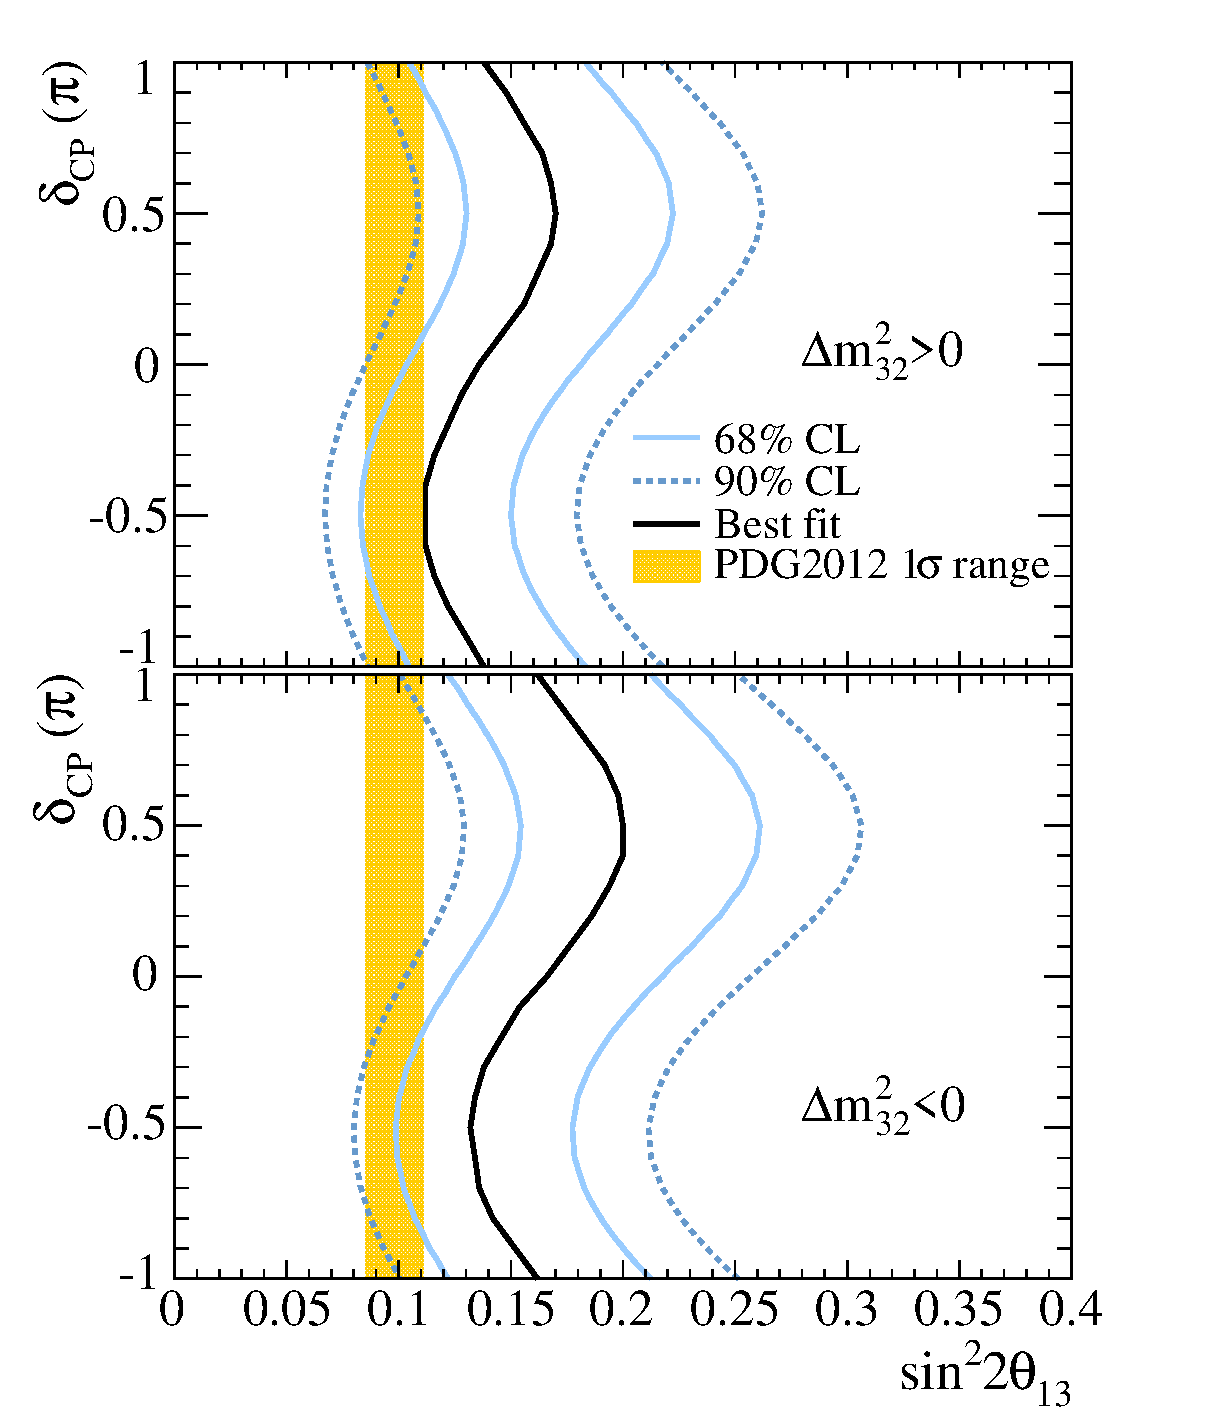
\includegraphics[width=7.5cm]{images/t2k/nue_appearance_Theta13Delta_contour.eps}
  \caption{The 68$\%$ and 90$\%$ confidence level allowed regions for $\sin^22\theta_{13}$ as a function of $\textrm{\delta}_{\textrm{CP}}$ for normal hierachy (top) and inverted hierarchy (bottom)  The solid line represents the best fit $\sin^22\theta_{13}$ for a given $\textrm{\delta}_{\textrm{CP}}$.  The shaded region shows the average $\theta_{13}$ provided by the reactor constraint~\cite{PhysRevLett.112.061802}.}
  \label{fig:NueAppearanceContour}
\end{figure}


\section{T2K beam}
\label{sec:T2KBeam}
The T2K neutrino beam is generated by J-PARC's accelerator complex which produces a 30 GeV proton beam which is fired at a fixed graphite target.  The final states particles of interactions with the target are predominately charged pions which decay to produce the neutrino beam.  Surrounding and behind the graphite target are a set of magnetic horns which focus the pions into a beam, resulting in a focused neutrino beam after the hadrons have decayed.

\subsection{Accelerator complex}
\label{subsec:AcceleratorComplex}
The J-PARC acclerator complex consists of three sections: the LINnear ACcelerator (LINAC), the Rapid-Cycling Synchotron (RCS) and the Main Ring synchotron (MR).  Production of the proton beam starts at the LINAC where H$^-$ anions are accelerated to 181 MeV which are subsequently converted to h$^+$ ions via charge-stripping foils at the RCS injection point.  With a 25 Hz cycle, the ions are further accelerated by the RCS to 3 GeV with two bunches per cycle.  Roughly 5$\%$ of the proton bunches are fed into the MR where the final acceleration to 30 GeV occurs in bunches of eight.  Extraction of the bunches occurs at two points for different experiments.  For T2K, all eight bunches are extracted in a single turn by five kicker magnets and aimed down the neutrino beamline to the graphite target.  The extraction of all eight bunches forms a single beam spill with a width of 5 $\mu$sec.  The tight structure of the beam spills is vital for background discrimination in the downstream detectors.

\subsection{Neutrino beamline}
\label{subsec:NeutrinoBeamline}

\begin{figure}
  \centering
  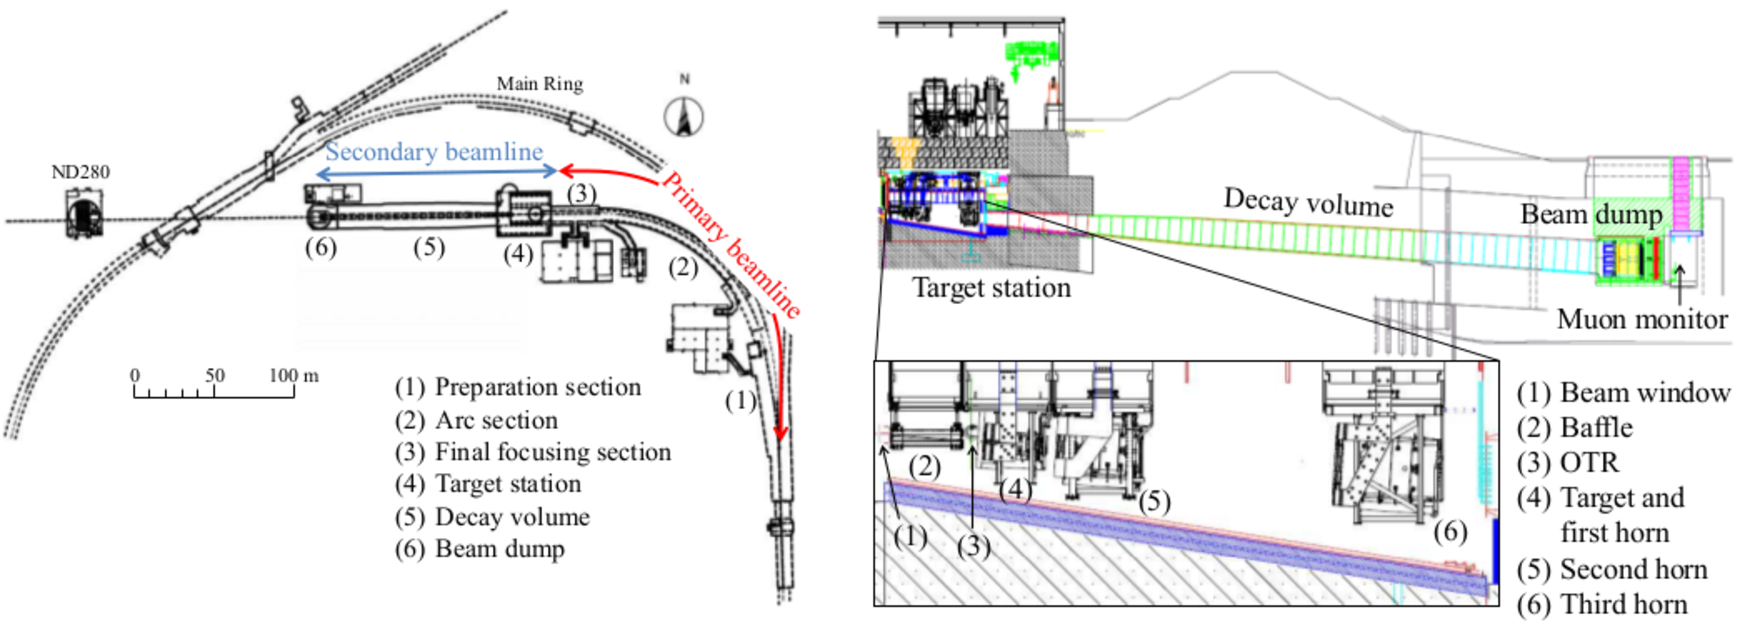
\includegraphics[width=15cm]{images/t2k/neutrino_beamline.pdf}
  \caption{A schematic of the T2K neutrino beamline (left) and a side view of the secondary beamline (right).}
  \label{fig:NeutrinoBeamline}
\end{figure}

The neutrino beamline (NU) is split into a primary and secondary beamline, a schematic of which is shown in Fig.~\ref{fig:NeutrinoBeamline}.  The primary beamline consists of a preparation section, an arc section and a focussing section.  The preparation section uses 11 normal conducting magnets to tune the proton beam for entry into the arc section where the proton beam is bent to its intended direction.  As will be discussed in more detail in section~\ref{subsec:OffAxisBeam}, the axis of the beam is 2.5$^\circ$ away from SK.  The final focussing sections then guides the proton beam into the secondary beamline and the graphite target.
\newline
Sound performance of the proton beam is vital for stability of the T2K neutrino beam.  To ensure such performance, the primary beamline is equipped with a suite of monitors to measure the position, profile, loss and intensity of the proton beam.  The beam position is measured by 21 electrostatic monitors (ESMs) which consists of four cylindrical electrodes surrounding the beam.  The asymmetry of the beam is measured by the induced current in the electrodes is used to infer the position in a non-destructive manner.  Segmented secondary emission monitors (SSEMs) are used to measure the beam loss.  Each SSEM has an anode foil sandwiched between two titanium foil strips.  Protons interact with the strips causing an emission of electrons which electrically drift inducing a current in the strips.  The charge distribution is used to reconstruct the profile.  The beam loss monitors (BLMs) are Ar-CO$_2$ filled wire proportional counters and are used to for beam loss.  The intensity of the beam is measured by five current transformers (CT) which consist of a 50-turn toroidal coil around a ferromagnetic coil.  Passage of the beam induces a current in the coil which is used to infer the number of protons in the spill.  The final CT (CT5) is positioned at the end of the focussing section of the primary beamline and is used to count the number of protons incident on the graphite target.  The accumulated number of protons on target (POT) is used as a metric for the data collected by T2K.  The total POT accumulated so far by T2K is shown in Fig.~\ref{fig:POTHistory}.
\begin{figure}
  \centering
  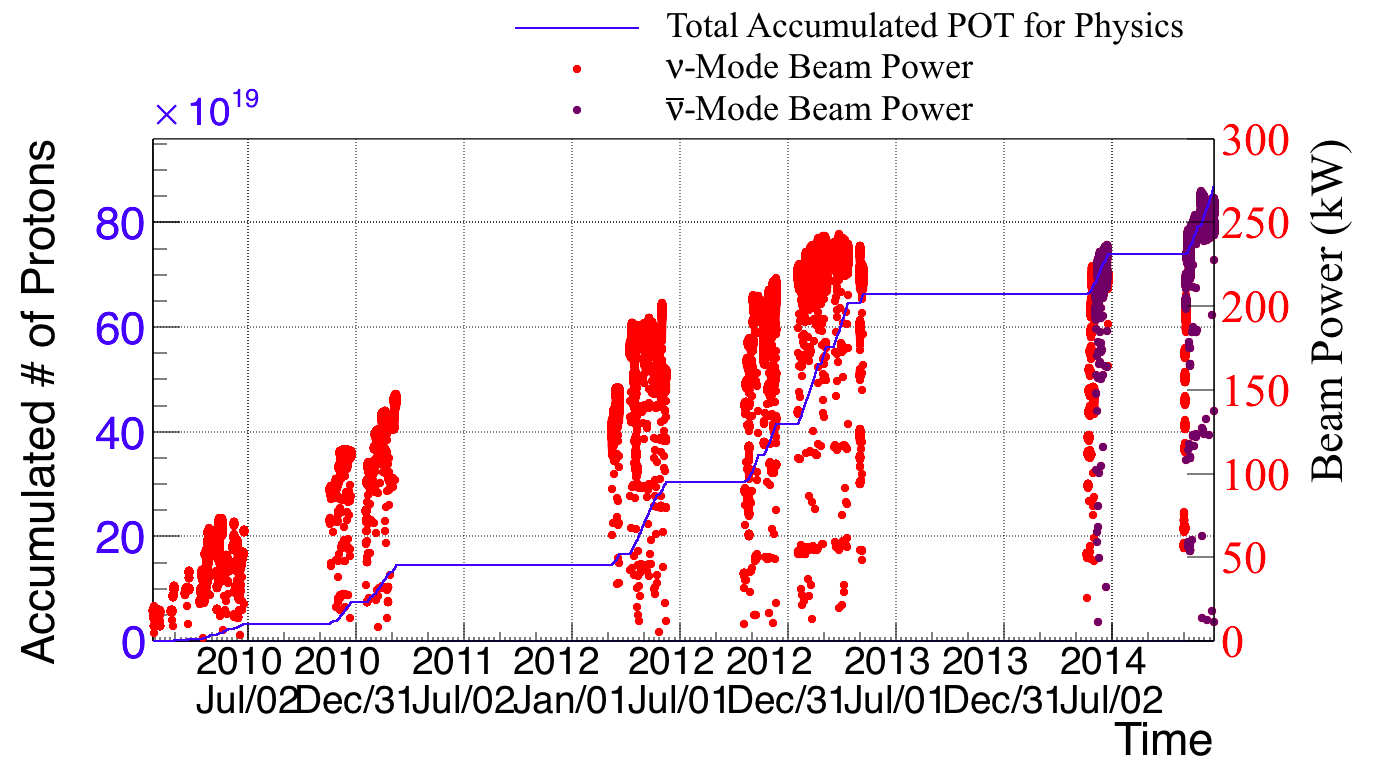
\includegraphics[width=15cm]{images/t2k/pot_history.png}
  \caption{The POT recorded by CT5 as a function of time (blue line) and the recorded beam power in $\nu$ running mode (red dot) and $\bar{\nu}$ running mode (purple dot).}
  \label{fig:POTHistory}
\end{figure}
\newline
The secondary beamline consists of the graphite target, a set of magnetic focusing horns, a decay pipe and a beam dump.  A schematic for the secondary beamline is shown in Fig.~\ref{fig:NeutrinoBeamline}.  The graphite target is a 2.6 cm diameter and 91.4 cm long rod which is surrounded by a 2 mm thick graphite tube and a 0.3 mm titanium case.  The proton-graphite interactions produce charged pions and kaons which are focussed by three magnetic horns, one of which surrounds the target.  The magnetic horns consist of two coaxial conductors which generate a magnetic field with a strength inversely proportional to the distance from the beam axis.  The current direction in the magnetic horns causes the induced field to focus or deflect particles depending on their charge sign.  This simple control allows T2K to operatre in $\nu$ or $\bar{\nu}$ beam mode.  The focused mesons then travel down a decay pipe filled with Helium to reduce pion absorption.  It is here that the mesons decay to produce the neutrinos used as the T2K beam.  To stop measurement contamination, other decay products must be stopped before reaching the downstream detectors.  So, a 75 ton graphite beam dump is positioned at the end of the decay volume.  The beam dump stops almost all non-wanted decay products, with only 5 GeV or above muons successfully propagating through.  As the muons are generally simultaneously produced with the beam neutrinos, measurements of the muon can be used to monitor the direction of the neutrino beam.  To do this, a muon monitor (MUMON) is installed at the downstream end of the beam dump.

\subsection{Off-axis beam}
\label{subsec:OffAxisBeam}
The kinematics of the pion decays dictate the energy spectrum shape of the neutrinos.  Specifically, the peak width of the neutrino energy narrows and shifts as an observer moves off-axis from the pions trajectory.  As the pions are the neutrino parents in the T2K beam, the same effect can be seen by moving off-axis from the neutrino beam.  This effect is illustrated in Fig.BLAH.  By positioning T2K's baseline detectors at 2.5$^\circ$ off-axis, it is possible to align the neutrino beam's peak energy with the first oscillation maximum for the $\nu_\mu$ disappearance channel.  Separately, an off-axis configuration reduces the beam's unwanted high energy tail, improving sensitivity to $\nu_e$ appearance and $\nu_\mu$ disappearance.


\section{Near detector complex}
\label{sec:NearDetectorComplex}
Stuff about comples

\subsection{Multi-Pixel Photon Counter}
\label{subsec:MPPC}
MPPCs

\subsection{INGRID}
\label{subsec:INGRID}
Stuff about INGRID

\subsection{ND280}
\label{subsec:ND280}
ND280 time

\subsubsection{The fine grain detectors}
\label{subsubsec:FGD}
FGDS

\subsubsection{The time projection chambers}
\label{subsubsec:TPC}
TPCs

\subsubsection{The $\pi^0$ detector}
\label{subsubsec:pi0detector}
Here is ref for \ref{subsubsec:TPC}
pi0

\subsubsection{The electromagnetic calorimeters}
\label{subsubsec:ecal}
The beasts

\subsubsection{The side muon range detector}
\label{subsubsec:smrd}
Why bother?

\subsection{The far detector}
I mean SK



